\section{Current Contributions}

\subsection{Proof of Concept}

%\begin{figure}[!b]
%   \begin{center}
%      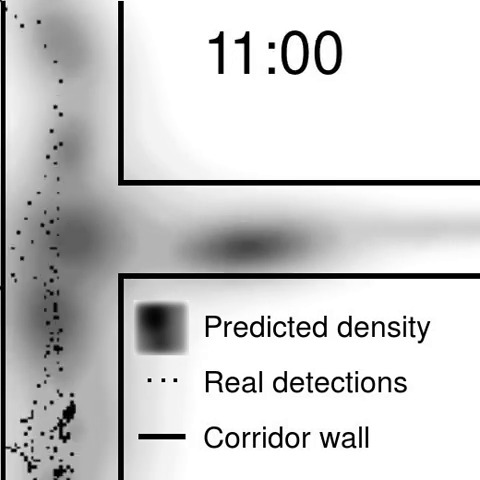
\includegraphics[width=0.3\columnwidth]{fig/corridor_0}
%    \hfill
%      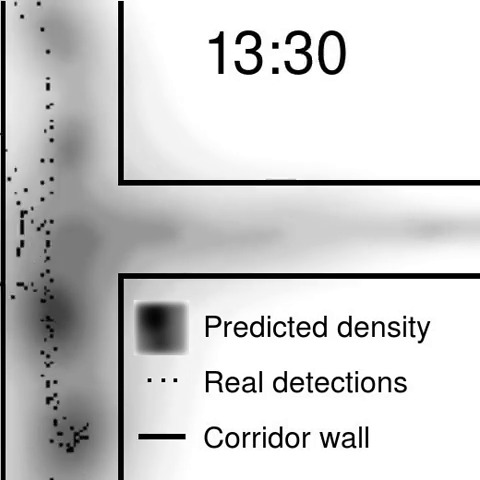
\includegraphics[width=0.3\columnwidth]{fig/corridor_1}\\\vspace{5mm}
%      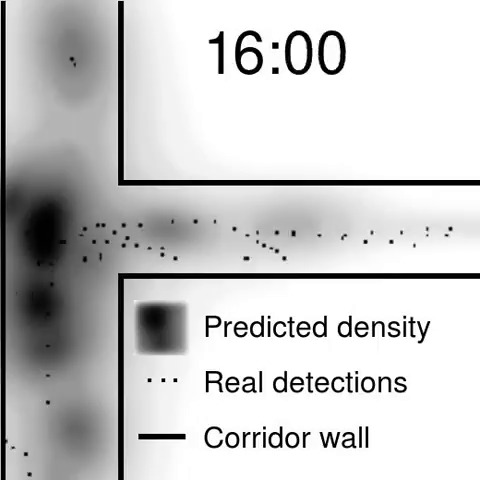
\includegraphics[width=0.3\columnwidth]{fig/corridor_2}
%    \hfill
%      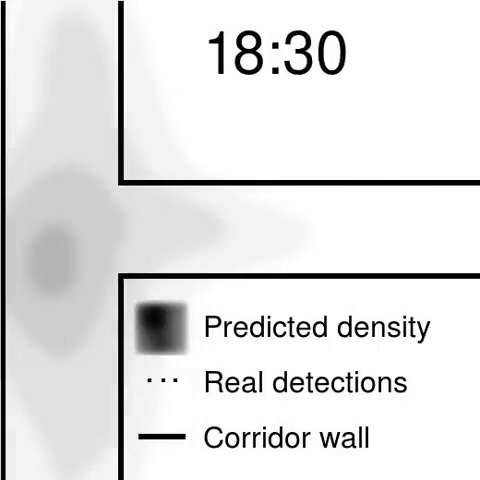
\includegraphics[width=0.3\columnwidth]{fig/corridor_3}
%      \caption{Screen grab from the video available at~\url{https://youtu.be/4SW4j7DDxYE}.\label{fig:video}}
%   \end{center}
%\end{figure}



\begin{itemize}
    \item T.~Vintr, S.~Molina, J.~Fentanes, G.~Cielniak, T.~Duckett, and T.~Krajn{\'i}k, ``Spatio-temporal models for motion planning in human-populated environments,'' in \emph{Student Conference on Planning in Artificial Intelligence and Robotics}, 2017.
\end{itemize}

In \cite{vintr2017spatiotemporal} we proposed a concept of modelling human activities over time in their natural environment.
We hypothesised that there are some patterns of human behaviour over the timeline.
As these patterns are derived from the routines and habits of humans, they show periodical and continuous nature.
We also hypothesised that there are no or negligible trends in these patterns due to the nature of human habits. 
%Let us consider these examples to explain periodicity and continuity of human behaviour:
Let us consider these examples form [mesas] to explain the periodicity and continuity of human behaviour:

%... copy from mesas ...
\begin{itemize}
    \item human  behaviour is very similar during every morning as opposed to the difference in behaviour during the morning and afternoon of one randomly chosen day,
    \item human behaviour five minutes before midnight and five minutes after midnight could be probably very similar, although we compare behaviour in two different days,
    \item contrary to that, human behaviour during Sunday afternoon is probably different from behaviour on Monday afternoon.
\end{itemize}
%... end ...

Such periodical behaviour is not only forced by natural physiological demands like fatigue or hunger, but also by social demands like regular working hours or the compulsory education system. 

To create the model of the time-dependent patterns of human behaviour, we need to classify detected events into the statistically describable classes.
As the timeline is continuous and it is not possible to repeat the experiment at the same time, the timeline is not suitable as a domain for time-dependent feature parameters estimation, especially for rare events.
The conventional approach to this task, known as time series forecasting, is to divide time-dependent events into three different components - a trend, seasonal and cyclic patterns - and analyse them separately \cite{gould2008forecasting}.
The cyclic patterns are non-predictable changes in the time series, seasonal patterns are the periodical changes, and the trend is continuous growth or decline of measured values.
To model human behaviour with the assumption of high periodicity and no trend, but with the accent to the continuity, we not only find and model dominant periodicities but also project timeline into a new multidimensional vector space.
In particular, we project every chosen periodicity into a $2d$ circle in the way, that every pattern that occurs periodically appears in the same position in this circle.
By this projection we address two issues:
\begin{itemize}
    \item the time domain is constrained, and therefore it is possible to estimate distribution parameters of the time-dependent periodical patterns,
    \item and the continuity remains.
\end{itemize}

\subsubsection{Time Projection in Detail}
%
\begin{figure}[!h]
   \begin{center}
      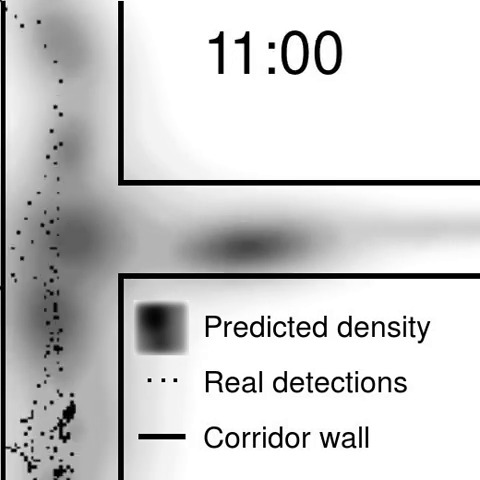
\includegraphics[width=0.24\columnwidth]{fig/corridor_0}
      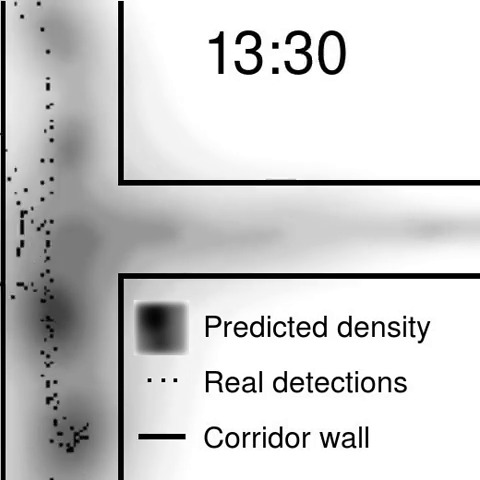
\includegraphics[width=0.24\columnwidth]{fig/corridor_1}
      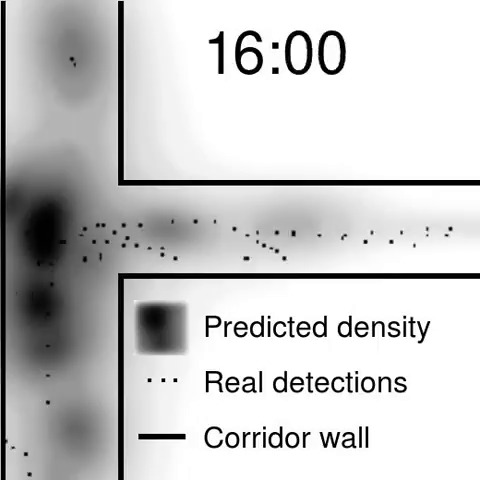
\includegraphics[width=0.24\columnwidth]{fig/corridor_2}
      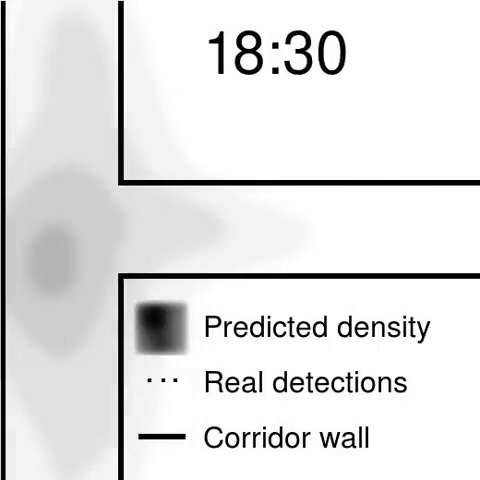
\includegraphics[width=0.24\columnwidth]{fig/corridor_3}
      \caption{Predicted people occurrence over a T-shaped corridor during different parts of the day. Screen grab from the video available at~\url{https://youtu.be/4SW4j7DDxYE}.\label{fig:video}}
%      \caption{Predicted people occurrence over a T-shaped corridor, see video at \url{https://youtu.be/4SW4j7DDxYE}.\label{fig:video}}
   \end{center}
\end{figure}

To prove this concept we used data of human positions during two days collected at the corridors of the School of Computer Science at the University of Lincoln.

%... !!! copy from pair ...
Data collection was performed by a mobile robot equipped with a Velodyne 3d laser range-finder.
The robot was placed at a T-shaped junction so that its laser range-finder was able to scan the three connecting corridors simultaneously.
To detect and localise people in the 3d point clouds provided by the scanner, we used an efficient and reliable person detection method~\cite{yan2017online}.
Each day contains approximately $28000$ entries, which correspond to hundreds of people walking or standing in the monitored corridors.
%... !!! end ...

The dataset consists of vectors $\left(x, y, t\right)$.
For the sake of simplicity we chose only one periodicity $T = 86400 s$ (one day), and project these vectors into the extended vector space in this way: $\left(x, y, t\right) \rightarrow \left(x, y, \cos\frac{2\pi t}{T}, \sin\frac{2\pi t}{T}\right)$.
Then we modelled the distribution by the Gustafson--Kessel Algorithm~\cite{gustafson1979fuzzy} with the number of clusters $k=30$.

\subsubsection{Conclusion}

We visualised this model of "distribution" of people at corridors in the form of a video that can be found online at [nefunkcni odkaz].
Every video frame, Figure~\ref{fig:video}, consists of $5$ minutes time frame reconstruction and the whole video consists of two days.
We can see that the model changes over time and respects corridor boundaries. 
We proved that this concept is functional.




\subsection{Warped Hypertime}

\begin{itemize}
    \item Spatiotemporal models of human activity for robotic patrolling (mesas)
\end{itemize}

\begin{figure}[!t]
\begin{center}
    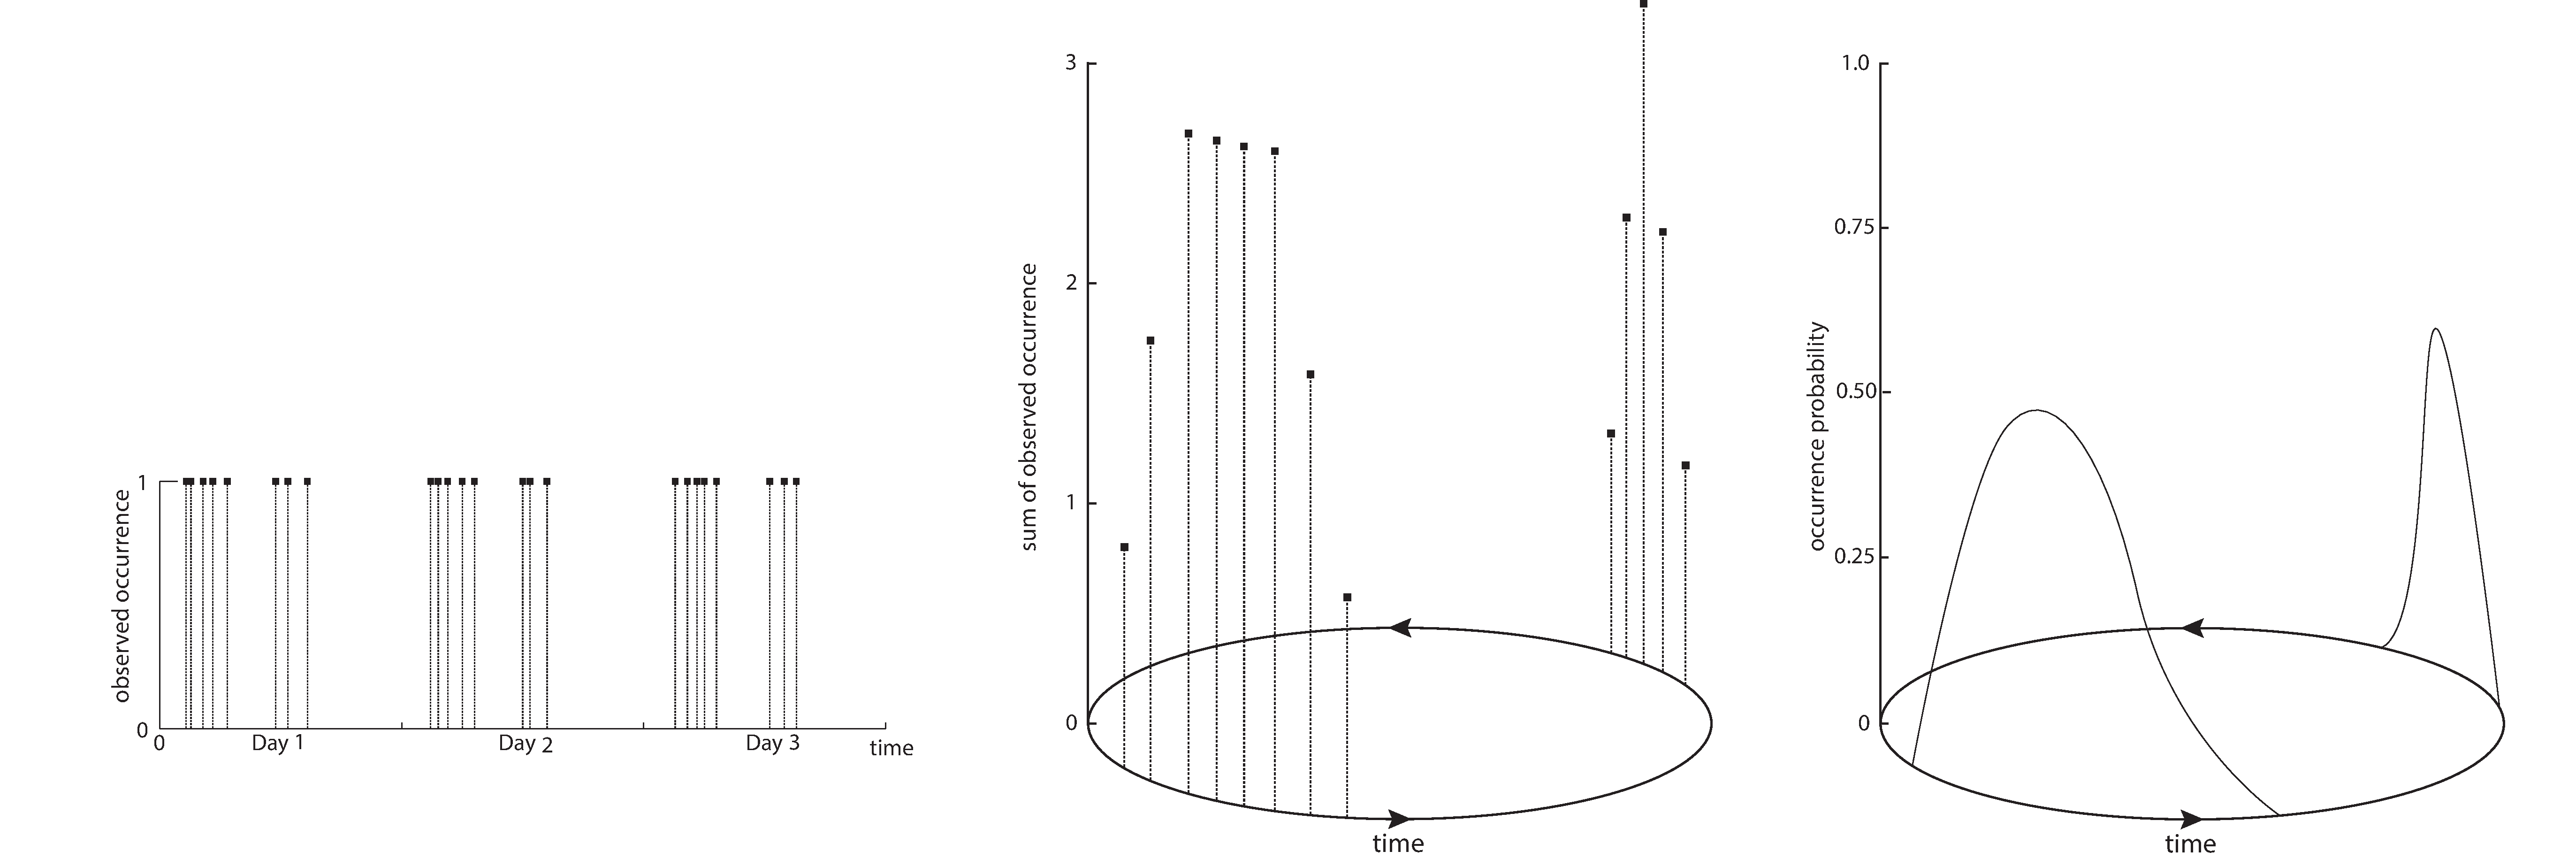
\includegraphics[width=1.0\columnwidth]{fig/hypertime_graph}
    \caption{Example of the warped hypertime projection. Positive detections during three days are projected into a warped hypertime with a one day period. The parameters of the distribution of a random time-dependent phenomenon that exhibit a periodic behaviour can be easily estimated, courtesy of [JFSS].\label{fig:hypertime}}

\end{center}
\end{figure}



The aim of the method presented in [mesas] was to create a model of human behaviour and detect anomalous events. 
We already showed that it is possible to extend the vector space of measured events by one circle, see Fig.~\ref{fig:hypertime}.
In this article, we hypothesised that it is possible to extend vector space with multiple circles and model the distribution of patterns matching different periodicities over such vector space.
To prove the concept of multiple circles extension we chose to: 
\begin{itemize}
    \item analyse the time series of human detections consisting of values one (human present) and zeros (human not present) over $18$ weeks, 
    \item and compare our approach to the FreMEn, the Frequency Map Enhancement method \cite{krajnik2017fremen} specially developed to model binomial time series, and Prophet \cite{taylor2018forecasting}, the open source, time series analysis tool created by Facebook.
\end{itemize}
%We call the projection of time into the multiple circles Warped Hypertime, WHyTe.

\subsubsection{Creation of Warped Hypertime}\label{sec:whyte}

%... copy from mesas ...
%Let us have time series $R\left(t_{i}\right)$, $i = 1 \ldots n$, where $R\left(t_{i}\right) = 1$ when the sensor detects an occurrence of the studied phenomenon and $R\left(t_{i}\right) = 0$ otherwise.
%Then we use the spectral analysis to find periodicities in the data. Specifically, we will use the method derived from the Frequency Map Enhancement \cite{krajnik2017fremen}.
%This method is suitable to analyse time series with binary data, and it is robust to missing values.
%For every considered period $T_{\tau}$, $\tau = 1 \ldots \Upsilon$, corresponding to the frequency ${f}_{\tau} = 1 / T_{\tau}$ we calculate a component of the frequency spectrum
%
%\begin{equation}\label{eq:components}
%\gamma_{\tau} = \frac{1}{n} \sum_{i = 1}^{n} (R\left(t_{i}\right)-\mu)e^{(-1j)t_{i}{f}_{\tau}2\pi},
%\end{equation}
%
%\noindent where $\mu = \frac{1}{n} \sum_{i = 1}^{n} R\left(t_{i}\right)$, sort them in descending order and return corresponding periods ordered accordingly.
%... end ...
%
%For every chosen period $T_{\tau}$ and for each $t_i$ of the original measured data we can create $2d$ warped hypertime (Fig.~\ref{fig:hypertime}) as follows:
%
%\begin{equation}
%t_i \rightarrow \left(\cos{\frac{2\pi t_{i}}{T_{\tau}}}, \sin{\frac{2\pi t_{i}}{T_{\tau}}}\right),
%\end{equation}
%%
%where warped hypertime $\left(\cos{\frac{2\pi t_{i}}{T_{\tau}}}, \sin{\frac{2\pi t_{i}}{T_{\tau}}}\right)$ forms a circle in $2d$ plane which represent the periodicity and continuity of the occurences.
%The time values of occurrences and non-occurrences with the similar position relative to periodicity $T_{\tau}$ are projected on the similar position on the circle.
%


\begin{figure}[!t]
\begin{center}
    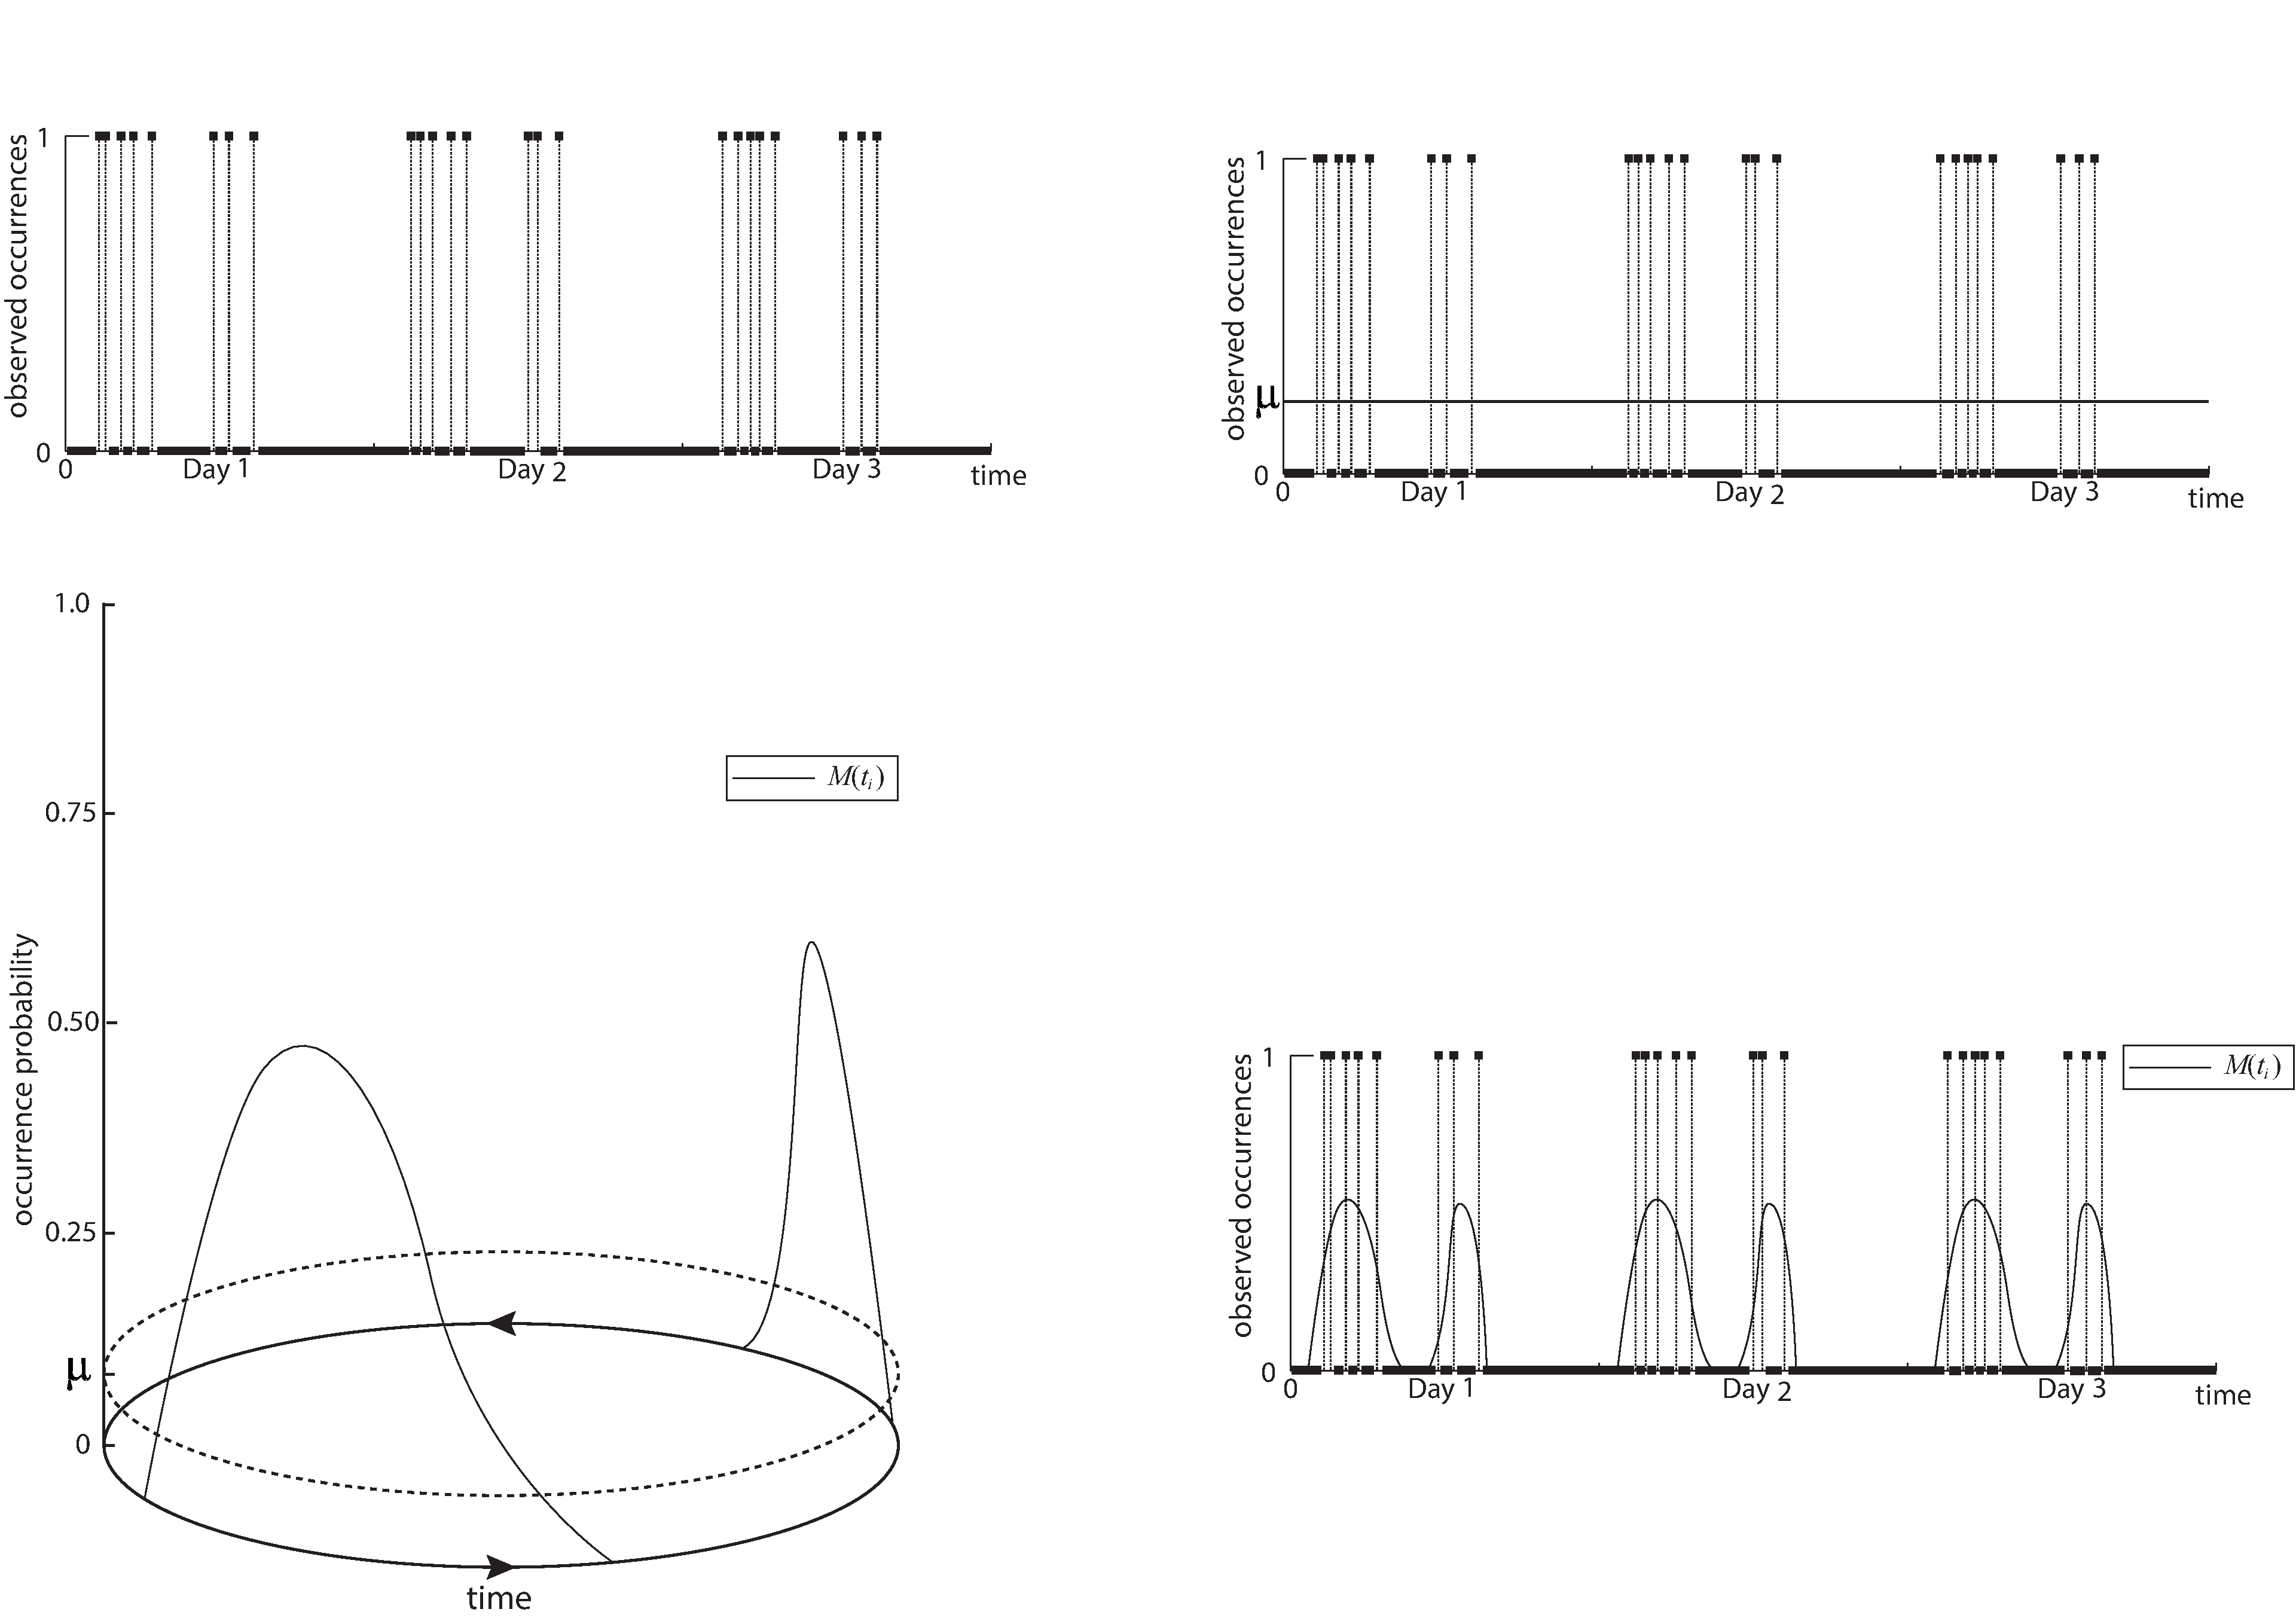
\includegraphics[width=1.0\columnwidth]{fig/hypertime_graphs_a}
    \caption{Warped hypertime iterations: The method inputs are observed occurrences of a given phenomenon over time (top left). Then, a model of the data is established (top right). Then, a dominant frequency of the model error is found by Eq.~\ref{eq:components}, the data points are projected onto a unit circle, and their distribution is modelled (bottom left). The model is then compared to the original data again (bottom right) and the process is repeated until the model error keeps decreasing, courtesy of [JFSS].\label{fig:whyte}}

\end{center}
\end{figure}



Let us have time series $R\left(t_{i}\right)$, $i = 1 \ldots n$, where $R\left(t_{i}\right) = 1$ for detected and $R\left(t_{i}\right) = 0$ for not detected occurrence of the studied phenomenon in the time $t_{i}$.
Then we apply the spectral decomposition method derived from the Frequency Map Enhancement \cite{krajnik2017fremen} on this time series to find prominent spectral components.
For every considered period $T_{\tau}$, $\tau = 1 \ldots \Upsilon$, corresponding to the frequency ${f}_{\tau} = 1 / T_{\tau}$ we calculate a component of the frequency spectrum

\begin{equation}\label{eq:components}
\gamma_{\tau} = \frac{1}{n} \sum_{i = 1}^{n} (R\left(t_{i}\right)-M\left(t_{i}\right))e^{(-1j)t_{i}{f}_{\tau}2\pi},
\end{equation}

\noindent where $M\left(t_{i}\right)$ is the actual model of the time series (for no previous model, $M\left(t_{i}\right)$ is the estimation of the expected value: $M\left(t_{i}\right) = \mu = \frac{1}{n} \sum_{i = 1}^{n} R\left(t_{i}\right)$), see Figure \ref{fig:whyte}, sort them in descending order and return corresponding periods ordered accordingly.

For every chosen period $T_{\tau}$ and for each $t_i$ of the original measured data we can create $2d$ warped hypertime (Fig.~\ref{fig:hypertime}) as follows:

\begin{equation}
t_i \rightarrow \left(\cos{\frac{2\pi t_{i}}{T_{\tau}}}, \sin{\frac{2\pi t_{i}}{T_{\tau}}}\right),
\end{equation}
%
where warped hypertime $\left(\cos{\frac{2\pi t_{i}}{T_{\tau}}}, \sin{\frac{2\pi t_{i}}{T_{\tau}}}\right)$ forms a circle in $2d$ plane which represent the periodicity and continuity of the occurences.
The time values of occurrences and non-occurrences with a similar position relative to periodicity $T_{\tau}$ are projected on a similar position on the circle.

During the iterative process, we extend the extended vector space with other couples of dimensions.
Such projection of $t_i$ will be denoted ${}^{@}\mathbf{t}_{i},$ where:
%
\begin{equation}\label{eqn:extension}
    {}^{@+1}\mathbf{t}_{i} = \left({}^{@}\mathbf{t}_{i}, \,\cos{\frac{2\pi t_{i}}{T_{\tau_{@+1}}}}, \, \sin{\frac{2\pi t_{i}}{T_{\tau_{@+1}}}}\right),
\end{equation}
%
in particular ${}^{2}\mathbf{t}_{i} =\left({}^{1}\mathbf{t}_{i}, \,\cos{\frac{2\pi t_{i}}{T_{\tau_2}}}, \, \sin{\frac{2\pi t_{i}}{T_{\tau_2}}}\right) =  \left(\cos{\frac{2\pi t_{i}}{T_{\tau_1}}}, \, \sin{\frac{2\pi t_{i}}{T_{\tau_1}}}, \,\cos{\frac{2\pi t_{i}}{T_{\tau_2}}}, \, \sin{\frac{2\pi t_{i}}{T_{\tau_2}}}\right),$ and
${}^{1}\mathbf{t}_{i} = \left(\cos{\frac{2\pi t_{i}}{T_{\tau_1}}}, \, \sin{\frac{2\pi t_{i}}{T_{\tau_1}}}\right)$.
We call the projection of time into the multiple circles Warped Hypertime, WHyTe.




\subsubsection{Creation of the Model}\label{sec:modelWhyte}

We assume that there exists a mixture of distribution of the time-dependent events of the measured phenomenon over the warped hypertime.
To find the model $M(t_{i})$ we apply the Expectation Maximisation algorithm for estimating Gaussian Mixture Models (EM GMM) on the projected time line ${}^{@}\mathbf{t}_{i}$ and create the estimation of of the mixture of the distributions:

\begin{equation}\label{eq:modelWHyTe}
{}^{@}M({}^{@}\mathbf{t}_{i}) =  \sum_{j=1}^{c}{\alpha_j\,u_{i,j}\left({}^{@}\mathbf{t}_{i}, \mathbf{c}_{j}\right)},
\end{equation}
%
\noindent where $\alpha_{j}$ are cluster weights and $u_{i,j}$ is a membership function dependent on the distance between ${}^{@}\mathbf{t}_{i}$ and the $j$-th cluster centre $\mathbf{c}_{j}$.

The clustering methods expect that there are only occurrences in the dataset, but in our dataset, there are occurrences, non-occurrences and missing values.
To overcome the problem of missing values, we created two models, ${}^{@}M^{1}({}^{@}\mathbf{t}_{i})$ and ${}^{@}M^{0}({}^{@}\mathbf{t}_{i})$ of the occurrences and the non-occurrences.
Than the probability model ${}^{@}M^{*}({}^{@}\mathbf{t}_{i})$ was calculated as follows:

\begin{equation}\label{eq:probabilityWHyTe}
{}^{@}M^{*}({}^{@}\mathbf{t}_{i}) = \frac{{}^{@}M^{1}({}^{@}\mathbf{t}_{i})}{{}^{@}M^{1}({}^{@}\mathbf{t}_{i}) + {}^{@}M^{0}({}^{@}\mathbf{t}_{i})}.
\end{equation}

Then we have to project values ${}^{@}M^{*}({}^{@}\mathbf{t}_{i})$ into the corresponding positions $t_{i}$ in the time line and create the model $M(t_{i})$ of the time series $R(t_{i})$.
However, the parameters of the mix of distributions (\ref{eq:modelWHyTe}) are not estimated idealy and therefore 
%this projection is not straightforward, because the cluster weights $\alpha_{j}$ are meaningful in the warped hypertime but not in the time domain.
%Therefore 
it is usually necessary to normalize the projected values ${}^{@}M^{*}({}^{@}\mathbf{t}_{i})$ in the way, that $\sum^{n}_{i=1}{M(t_{i})} = \sum^{n}_{i=1}{R(t_{i})}$ over the training data:

\begin{equation}\label{eq:modelNormalisation}
M(t_{i}) = \frac{\sum^{n}_{i=1}{R(t_{i})}}{ \sum^{n}_{i=1}{{}^{@}M^{*}({}^{@}\mathbf{t}_{i})}}{}^{@}M^{*}({}^{@}\mathbf{t}_{i}).
\end{equation}






\subsubsection{Conclusion}
\begin{figure}[t!]
\begin{center}
    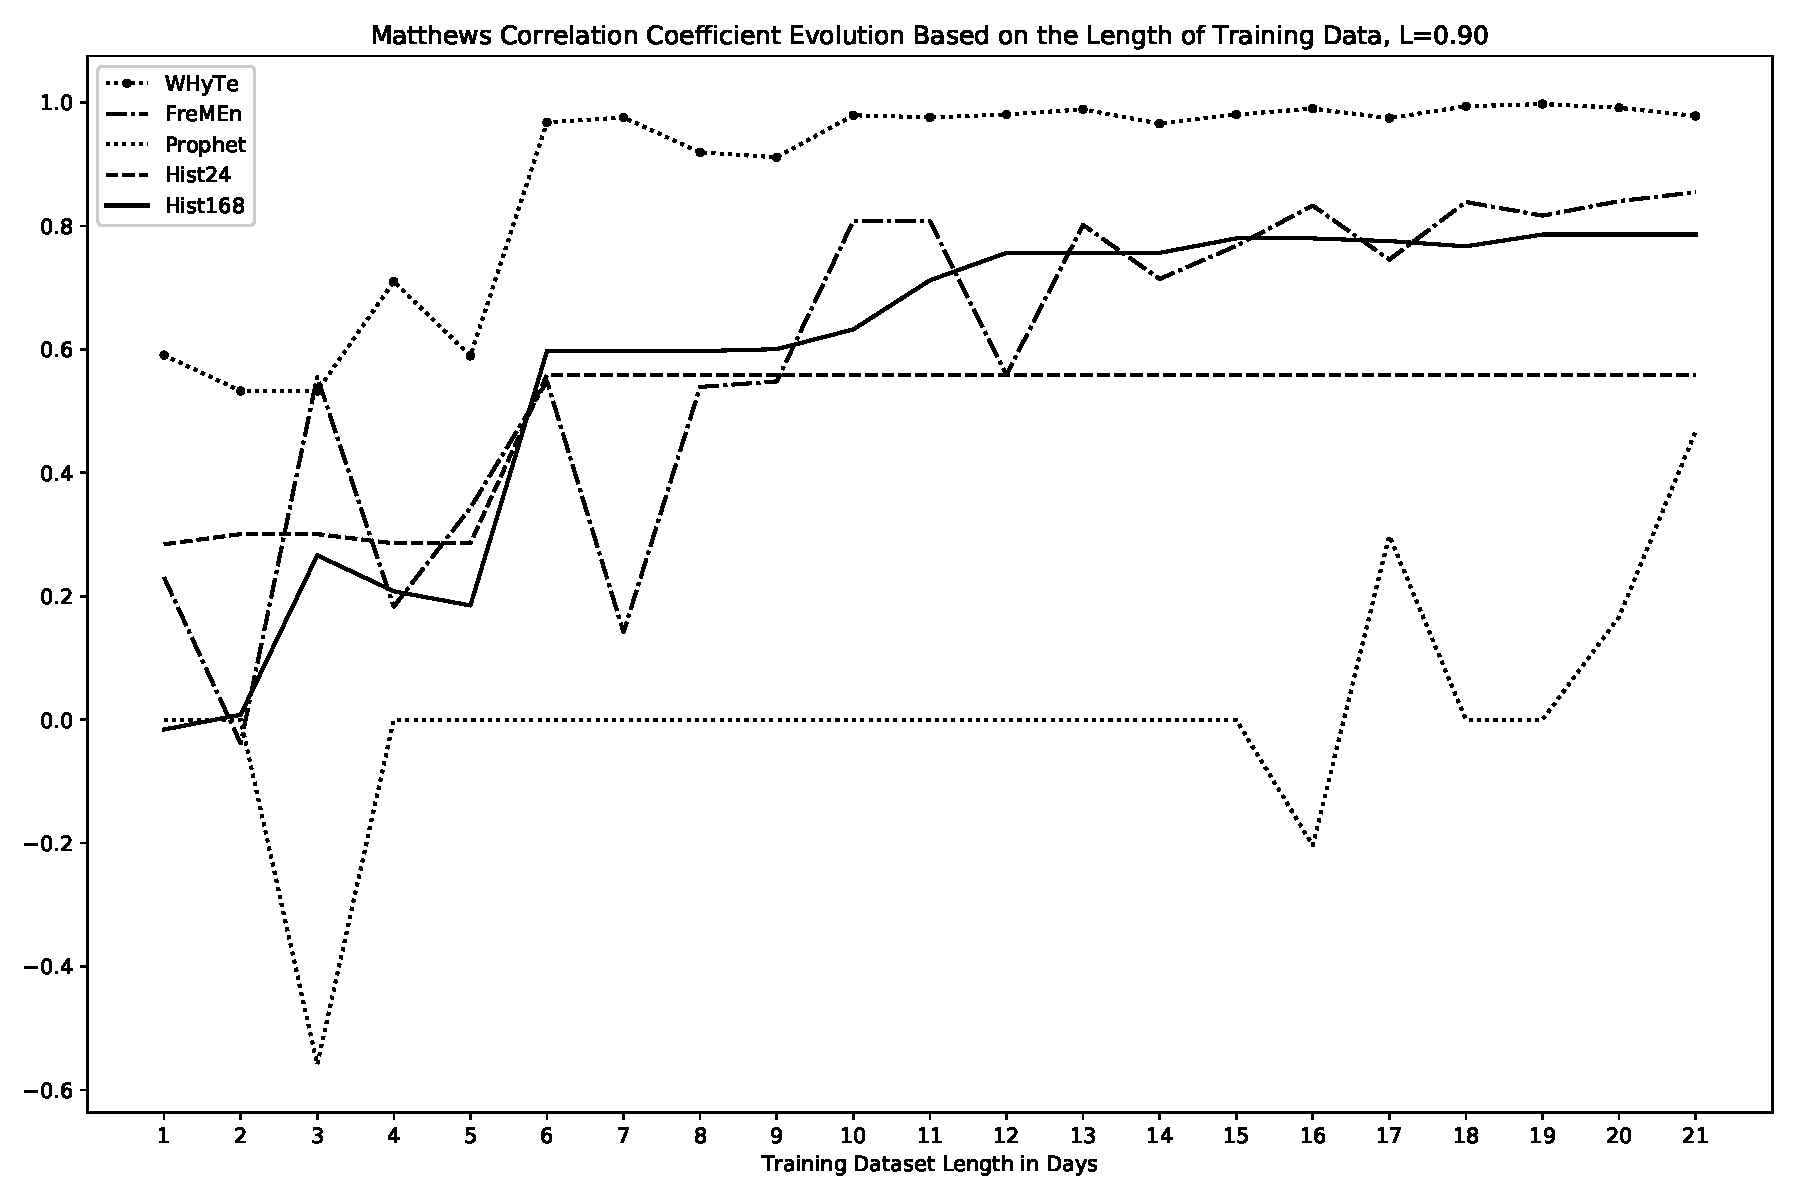
\includegraphics[width=1.0\columnwidth]{fig/mathew_graph_90}
    \caption{Evolution of Matthews correlation coefficient using significance level $\alpha=0.1$. On the x axis there are numbers of days used to train model, on the y axes are values of Matthews correlation coefficient $\left<-1;1\right>$. A coefficient of value $1$ means correct labelling of outliers by the corresponding method.   \label{graph:mathew90}}

\end{center}
\end{figure}

In [mesas] we compare the anomaly detection ability of model based on warped hypertime to other approaches, especially FreMEn \cite{krajnik2017fremen} and Prophet \cite{taylor2018forecasting}. 
It was successfully compared in multiple ways (Figure~\ref{graph:mathew90}): a number of days needed to learn the cor model, the correctness of anomaly detection deduced from Matthews correlation coefficient \cite{matthews1975comparison} and robustness to the choice of significance level.
We proved that it is possible to model patterns matching different periodicities by the projection of the timeline into the multidimensional warped hypertime.
It also proved our hypothesis, that it is possible to neglect trend in time series when modelling human behaviour.





\subsection{Warped Hypertime Space}

\begin{itemize}
    \item Spatio-temporal representation for long-term anticipation of human presence in service robotics (icra)
\end{itemize}

The aim of the method proposed in [icra] was to create a spatio-temporal model of human presence. 
The primary hypothesis is that it is possible to extend the space with the warped hypertime and create a model of frequencies over this projection.
We call this projection warped hypertime space, WHyTeS. 
We also hypothesise that model of frequencies over the hypertime space is less memory consuming than methods based on the grid.

%To create a model of frequencies, it is necessary to define a basic element of space-time above which is the unit frequency calculated. 
%The volume of the basic elements directly defines the resolution of the method.
To prove the concept of multiple time circles extension of the space, we create the model over the dataset collected at the corridors of the School of Computer Science at the University of Lincoln.
The dataset consists of the human detections at the T-shaped junction over three weeks.
We divided the dataset to the training part, consisting of two weeks of measurement and the test part consisting of two days from another week.
The model was then compared in the power of prediction to the known state of the art method FreMEn and histogram, which is the most popular approach in the robotics.

\subsubsection{Creation of Warped Hypertime Space}\label{sec:whytes}

%Neglecting spatial parts $\mathbf{x}_{i}$ of vectors $\left(\mathbf{x}_i, t_i\right)$, we can analyze periodicities of time series $R\left(t_{i}\right) = R\left(\mathbf{x}_i, t_i\right)$ according to the (\ref{eq:components}) and gain periods $T_{\tau}$ ordered by their influences.
%...copy from icra...
%Once we have identified and chose the dominant period $T_{\tau}$, we can extend the space with two extra dimensions.
%For each $\left(\mathbf{x}_i, t_i\right)$ of the original measured data in space-time, we calculate its projection into the space extended by warped hypertime as follows:
%
%\begin{equation}
%\left(\mathbf{x}_i, t_i\right) \rightarrow \left(\mathbf{x}_i, \cos{\frac{2\pi t_{i}}{T_{\tau}}}, \sin{\frac{2\pi t_{i}}{T_{\tau}}}\right),
%\end{equation}
%%
%During the iterative process we can extend the extended vector space with another two dimensions and create a more dimensional warped hypertime extension of the space. 
%Such projection of the measurements $\mathbf{x}_i$ obtained at time $t_i$ will be denoted ${}^{@}\mathbf{x}_{i},$ where:
%%
%\begin{equation}\label{eqn:extension}
%    {}^{@+1}\mathbf{x}_{i} = \left({}^{@}\mathbf{x}_{i}, \,\cos{\frac{2\pi t_{i}}{T_{\tau_{@+1}}}}, \, \sin{\frac{2\pi t_{i}}{T_{\tau_{@+1}}}}\right),
%\end{equation}
%%
%and ${}^{0}\mathbf{x}_{i} = \mathbf{x}_{i},$ ${}^{1}\mathbf{x}_{i} = \left(\mathbf{x}_{i}, \,\cos{\frac{2\pi t_{i}}{T_{\tau_1}}}, \, \sin{\frac{2\pi t_{i}}{T_{\tau_1}}}\right),$ ${}^{2}\mathbf{x}_{i} = \left(\mathbf{x}_{i}, \,\cos{\frac{2\pi t_{i}}{T_{\tau_1}}}, \, \sin{\frac{2\pi t_{i}}{T_{\tau_1}}}, \,\cos{\frac{2\pi t_{i}}{T_{\tau_2}}}, \, \sin{\frac{2\pi t_{i}}{T_{\tau_2}}}\right),$ etc.
%...end ...

Let us have spatio-temporal detections of occurrences and non-occurrences at time $\left(\mathbf{x}_i, t_i\right)$.
Neglecting spatial parts $\mathbf{x}_{i}$ of vectors $\left(\mathbf{x}_i, t_i\right)$, we can analyze periodicities of time series $R\left(t_{i}\right) = R\left(\mathbf{x}_i, t_i\right)$ according to the (\ref{eq:components}) and gain periods $T_{\tau}$ ordered by their influences.
We chose the dominant period $T_{\tau}$ and extended the space with two new dimensions.
Then we project every measurement $\left(\mathbf{x}_i, t_i\right)$ into the new vector space as follows:
%...copy from icra...

\begin{equation}
\left(\mathbf{x}_i, t_i\right) \rightarrow \left(\mathbf{x}_i, \cos{\frac{2\pi t_{i}}{T_{\tau}}}, \sin{\frac{2\pi t_{i}}{T_{\tau}}}\right),
\end{equation}
%
During the iterative process we can extend the extended vector space with another two dimensions and create a more dimensional warped hypertime extension of the space. 
Such projection of the measurements $\mathbf{x}_i$ obtained at time $t_i$ will be denoted ${}^{@}\mathbf{x}_{i},$ where:
%
\begin{equation}\label{eqn:extensionWHyTeS}
    {}^{@+1}\mathbf{x}_{i} = \left({}^{@}\mathbf{x}_{i}, \,\cos{\frac{2\pi t_{i}}{T_{\tau_{@+1}}}}, \, \sin{\frac{2\pi t_{i}}{T_{\tau_{@+1}}}}\right),
\end{equation}
%
and ${}^{0}\mathbf{x}_{i} = \mathbf{x}_{i},$ ${}^{1}\mathbf{x}_{i} = \left(\mathbf{x}_{i}, \,\cos{\frac{2\pi t_{i}}{T_{\tau_1}}}, \, \sin{\frac{2\pi t_{i}}{T_{\tau_1}}}\right),$ ${}^{2}\mathbf{x}_{i} = \left(\mathbf{x}_{i}, \,\cos{\frac{2\pi t_{i}}{T_{\tau_1}}}, \, \sin{\frac{2\pi t_{i}}{T_{\tau_1}}}, \,\cos{\frac{2\pi t_{i}}{T_{\tau_2}}}, \, \sin{\frac{2\pi t_{i}}{T_{\tau_2}}}\right),$ etc.
%...end ...



\subsubsection{Resolution and Model of Frequencies}\label{sec:resolution}

%The volume $b$ of the basic element of the space-time has to be chosen accordingly to the purposes of the model (for example $1$ squared meter hour $[m^{2}h]$). 
%Then we can create histogram $\mathbf{H}$ with bins of volume $b$.
%Spatio-temporal positions of bins are defined by vectors $\left(\mathbf{b}_{k}, t_{k}\right)$, where $k$ are meaningful indices.
%Vectors $\left(\mathbf{b}_{k}, t_{k}\right)$ should lie inside the area of bin, preferably in the spatio-temporal centers of bins.
%The values $v_{k}$ connected to each bin are than calculated as a sum of values $R\left(\mathbf{x}_i, t_i\right)$ assigned to every $\left(\mathbf{x}_i, t_i\right)$ that lies inside of the volume of the corresponding bin.
%Using the histogram $\mathbf{H}$, we modelled frequencies of measured phenomenon per chosen volume unit $b$ as follows:
%\begin{enumerate}
%    \item Assumming that every measure $R\left(\mathbf{x}_i, t_i\right)$ is one or zero,  apply a clustering method to ${}^{@}\mathbf{x}_{i}$ for every $\left(\mathbf{x}_i, t_i\right) : R\left(\mathbf{x}_i, t_i\right) = 1 $,
%    \item calculate centroids $\mathbf{c}_c$ and covariance matrices $\Sigma_{c}$ of every cluster, and membership $u_{i, c}$ of every ${}^{@}\mathbf{x}_{i}$ to every cluster, where $c$ is index of clusters,
%    \item using $\mathbf{c}_c$ and $\Sigma_{c}$ calculate membership $u_{k, c}$ of every ${}^{@}\mathbf{b}_{k}$ to every cluster,
%    \item calculate cluster weights $\alpha_{c}$ as
%\begin{equation}
%    \alpha_{c} = \frac{\sum_{i}u_{i, c}}{\sum_{k}u_{k, c}}
%\end{equation}\label{eqn:cluster_weights}
%    \item than function
%\begin{equation}\label{eqn:distribution}
%    \rho\left(\mathbf{x}_{0},t_{0}\right) = \sum_{j=1}^{c}{\alpha_j\,u_{0j}{}^{@}\mathbf{x}_{0}}
%\end{equation}
%estimates frequency of measured phenomenon in the neighbourhood with volume $b$ around $\left(\mathbf{x}_0, t_0\right)$.
%\end{enumerate}
%%
%The quality of the model is based on two parameters, the number of clusters and the set of chosen periodicities to create the hyper time.
%To find proper parameters, we create models with different parameters and chose the one with minimal overall differences between $\rho\left(\mathbf{b}_{k},t_{k}\right)$ and $v_{k}$.
%However, we did not find any elegant heuristic to estimate these parameters.

%In the recent research we used a different approach that does not need the assumption, that the measured values $R\left(\mathbf{x}_i, t_i\right)$ are integers:
%\begin{enumerate}
%    \item Create histogram $\mathbf{H}$ with bins of volume $b$,
%    \item project $\left(\mathbf{b}_{k}, t_{k}\right)$ into ${}^{@}\mathbf{b}_{k}$,
%    \item apply k-nearest neighbors regression \cite{altman1992introduction} as implemented in Scikit-learn \cite{scikit-learn}.
%\end{enumerate}
%
%Althought this model needs also two parameters, the set of chosen periodicities and number of neighbors to use for kneighbors queries, preliminary test indicate similar or better prediction power of gained models with lower computational time than earlier method.


Contrary to the previous task (subsection \ref{sec:modelWhyte}), the task is not to estimate the probability distribution of the presence of people in time, but to estimate the number of people in some area, i.e., to create a model of the frequency of people in the studied space-time [icra].
We estimate the parameters of the mixture of distributions of human occurrences over the warped hypertime space using EM GMM.
Then we project the probability model values ${}^{@}M({}^{@}\mathbf{x}_{i})$ back to the space-time and estimate the model of frequency.

We have to define a basic element of space-time above which is the unit frequency calculated. 
The volume $b$ of the basic elements directly defines the resolution (granularity) of the method, and it is necessary to define it according to the purposes of the model.
For example, choosing $b$ to be equal to $1$ squared meter hour $[m^{2}h]$ means, that the robot can ask, how many people will be present during the specific hour on the area of one square meter around the specific position). 

We create histogram $\mathbf{H}$ with bins of volume $b$ over the space-time, where any detection (either positive or negative) occurred.
Spatio-temporal positions of bins are defined by dheir centres $\left(\mathbf{b}_{k}, t_{k}\right)$, where $k$ is is a bin index.
%Vectors $\left(\mathbf{b}_{k}, t_{k}\right)$ should lie inside the area of bin, preferably in the spatio-temporal centers of bins.
The values $v_{k}$ associated with each bin are than calculated as a sum of values $R\left(\mathbf{x}_i, t_i\right)$ assigned to every $\left(\mathbf{x}_i, t_i\right)$ that lies inside of the volume of the corresponding bin.
Using the histogram $\mathbf{H}$, we modelled frequencies of measured phenomenon per chosen volume unit $b$ as follows:
\begin{enumerate}
    \item Assumming that every measurement $R\left(\mathbf{x}_i, t_i\right)$ is one or zero,  apply a clustering method to ${}^{@}\mathbf{x}_{i}$ for every $\left(\mathbf{x}_i, t_i\right) : R\left(\mathbf{x}_i, t_i\right) = 1 $,
    \item using a given clustering method, calculate centroids $\mathbf{c}_j$ and covariance matrices $\Sigma_{j}$ of every cluster, and membership $u_{i, j}\left({}^{@}\mathbf{x}_{i}, \mathbf{c}_{j}\right)$ of every ${}^{@}\mathbf{x}_{i}$ to every cluster $\mathbf{c}_{j}$, where $j = 1\ldots c$ is index of clusters,
    \item using $\mathbf{c}_j$ and $\Sigma_{j}$ calculate membership $u_{k, j}\left({}^{@}\mathbf{b}_{k}, \mathbf{c}_{j}\right)$ of every bin centre projection${}^{@}\mathbf{b}_{k}$ to every cluster $\mathbf{c}_{j}$,
    \item calculate cluster weights $\alpha_{j}$ as
\begin{equation}\label{eqn:clusterWeights}
    \alpha_{j} = \frac{\sum_{i}u_{i, j}}{\sum_{k}u_{k, j}},
\end{equation}
where $\sum_{j}u_{i, j} = 1$,
    \item than function
\begin{equation}\label{eqn:distribution}
    \rho\left(\mathbf{x}_{0},t_{0}\right) = \sum_{j=1}^{c}{\alpha_j\,u_{0j}\left({}^{@}\mathbf{x}_{0}, \mathbf{c}_{j}\right)}
\end{equation}
estimates frequency of measured phenomenon in the neighbourhood with volume $b$ around $\left(\mathbf{x}_0, t_0\right)$.
\end{enumerate}
%


The quality of the model is based on two parameters, the number of clusters $c$ and the set of chosen periodicities to create the hypertime.
To find proper parameters, we create models with different parameters and chose the one with minimal overall differences between $\rho\left(\mathbf{b}_{k},t_{k}\right)$ and $v_{k}$.
However, we did not find any elegant heuristic to estimate these parameters.


\begin{figure}[!t]
\begin{center}
    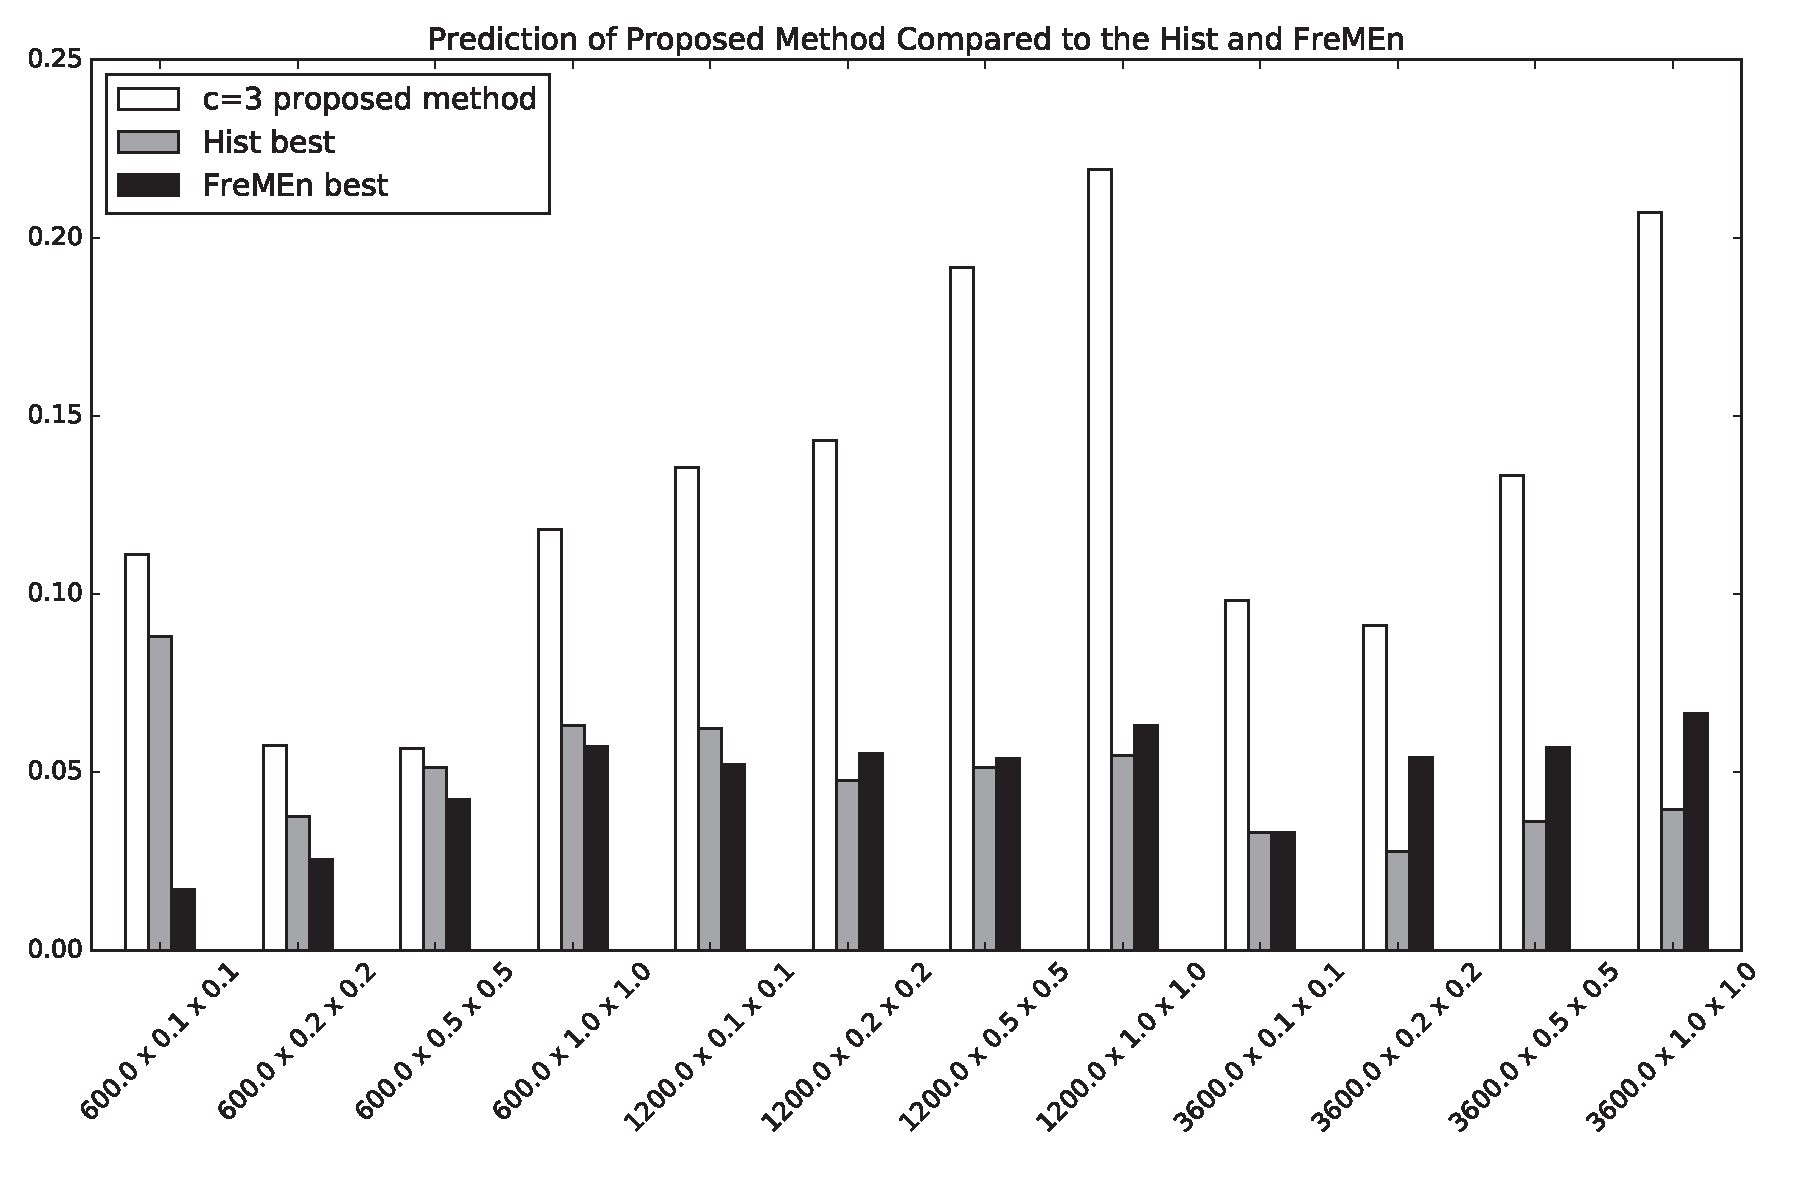
\includegraphics[width=1.0\columnwidth]{fig/ours3_hist_fremen.pdf}
    \caption{Comparison of predictive power of different methods. 
The graph shows the reduction of the prediction error compared to the \textit{Mean} model, which neglects the temporal properties of the people presence.
The indicated values ($y$-axes) are calculated using (\ref{eq:ratio}). 
On the $x$ axis, there are cell sizes or basic volumes.
White bar shows the prediction power of the proposed method using three clusters, grey bar Hist and black bar FreMEn.\label{graph:pedestrians}}
\end{center}
\end{figure}

\begin{table}[!b]
\caption{Memory Efficiency of Compared Methods}
\label{tab:ram}
%\resizebox{1.0\textwidth}{!}{%
\centering{
\begin{tabular}{ccccc}
\hline
\begin{tabular}[c]{@{}c@{}}resolution\\ {[}cm x cm{]}\end{tabular} & \begin{tabular}[c]{@{}c@{}}proposed method\\ c = 3, @ = 2\end{tabular} & \begin{tabular}[c]{@{}c@{}}FreMEn\\ f = 5\end{tabular} & \begin{tabular}[c]{@{}c@{}}Hist\\ h = 24\end{tabular} & Mean      \\ \hline
100 x 100                                                          & 1.7 KiB                                                                & 1.1 MiB                                                & 19.3 KiB                                              & 3.3 KiB   \\
50 x 50                                                            & 1.7 KiB                                                                & 4.4 MiB                                                & 307.3 KiB                                             & 12.9 KiB  \\
20 x 20                                                            & 1.7 KiB                                                                & 27.2 MiB                                               & 1.9 MiB                                               & 80.1 KiB  \\
10 x 10                                                            & 1.7 KiB                                                                & 108.9 MiB                                              & 7.7 MiB                                               & 320.1 KiB \\ \hline
\end{tabular}%
}
\end{table}

\subsubsection{Conclusion}

In [icra] we compared prediction power and computational and memory cost of the model of frequencies based on clustering over the warped hypertime space 
%... !!! copy of icra ... 
to three other spatio-temporal models. 
These three models represent the space in a discrete way - in particular, they associate each cell of the spatial 2d grid with a temporal model: 
\begin{itemize}
    \item \textit{Mean}, which is simply an average of the past measurements, 
    \item \textit{Hist}, which splits each day into $h$ intervals and predicts the number of occurrences as an average for the relevant time of a day, 
    \item \textit{FreMEn}, which extracts $f$ spectral components from the people occurrence history and uses these periodic components for future predictions.
\end{itemize}
As the corridor is T shaped, we decided to choose $c = 3$ number of clusters for a proposed method. 
Since the error of prediction is dependent on the partitioning used, we tested the method for grids of various cell sizes (basic volumes $b$) ranging from $0.1$ to $1.0$ meters and $10$ to $60$ minutes.
To better visualize the comparison of prediction capabilities of different methods on different resolutions (Figure ~\ref{graph:pedestrians}), we show the ratio between a root-mean-square deviation \cite{hyndman2006another} (RMSD) of prediction of every compared method to a RMSD of prediction gathered from the \textit{Mean}, i.e.,

\begin{equation}\label{eq:ratio}
ratio = 1 - \frac{RMSD_{method}}{RMSD_{Mean}}.
\end{equation}
%... !!! end ... 



We proved that it is possible to extend spatial dimensions by the warped hypertime and create the model of frequencies of a measured phenomenon over this projection.
We also proved that such a model is significantly more memory efficient, see Table \ref{tab:ram},  and therefore more scalable.
Moreover, contrary to other methods, it is not necessary to create a model for every required resolution.
The presented method can only store different sets of $\alpha_{j}$.  
The downside of this approach is its computational complexity.
FreMEn calculates a temporal model of all the grid cells in less than a minute, while our method built the spatio-temporal model in an hour (CPU Intel Core i7-5005U).



\subsection{Use Cases in Real Robot Systems}

\begin{itemize}
    \item T.~Krajnik, T.~Vintr, S.~Molina, J.~P. Fentanes, G.~Cielniak, and T.~Duckett, ``Warped hypertime representations for long-term autonomy of mobile robots,'' \emph{arXiv preprint arXiv:1810.04285}, 2018.
%    \item T.~Krajn{\'i}k, M.~Hanheide, T.~Vintr, K.~Kusumam, and T.~Duckett, ``Towards automated benchmarking of robotic experiments,'' in \emph{ICRA Workshop on  Reproducible Research in Robotics}, 2017.
\end{itemize}

In \cite{krajnik2018warped} we hypothesise that projection of the time-space into the warped hypertime space, and modelling spatio-temporal phenomena using clustering methods leads to more precise models compared to the discrete methods.
The idea behind this hypothesis lies in the assumption that the continuous model takes into consideration dependencies between
 the surroundings not only in the temporal \cite{tipaldi2013lifelong,rosen2016towards,kucner2013conditional,krajnik2017fremen} but also spatial meaning.
We created a set of four scenarios experiments \cite{krajnik2017towards}, which can be useful for task scheduling and planning~\cite{mudrova2015integrated}.
These experiments evaluate the predictive power of tested methods in the same way, and the evaluation tool is prepared for
 comparing different methods, that can be uploaded by any researcher from the robotic community \cite{krajnik2017towards}.

The list of scenarios is as follows:
\begin{enumerate}
    \item the door state
    \begin{itemize}
        \item a binary variable that indicates whether the doors are opened or closed during ten weeks,
        \item the methods have to predict the door state in the chosen times,
    \end{itemize}
    \item the topological localisation
    \begin{itemize}
        \item a large set of binary variables, each indicates visibility of selected point of interest from the $8000$ images,
        \item the methods have to predict the most probably visible points of interest in the specific times,
    \end{itemize}
    \item the velocity prediction
    \begin{itemize}
        \item a continuous variable, which indicates the time the robot needs to traverse a path in the human populate
d area,
        \item the methods have to predict the time to traverse the path in specific times,
    \end{itemize}
    \item and the human presence
    \begin{itemize}
        \item a three-dimensional variable, which indicates human detection (binary part) on the two-dimensional surface (two dimensional continuous part),
        \item the methods have to predict the frequency of people in a specific time and area.
    \end{itemize}
\end{enumerate}

\subsubsection{Conclusion}
%
%\begin{figure}[!h]
%   \begin{center}
%      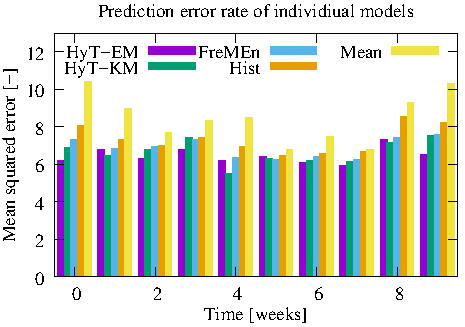
\includegraphics[width=0.24\columnwidth]{fig/door_graph}
%      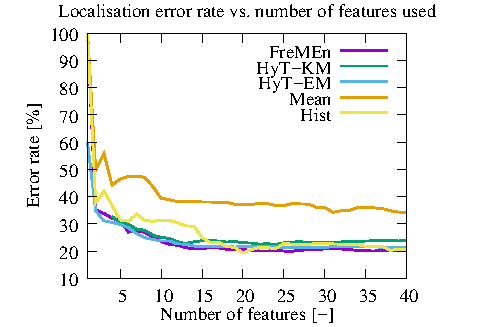
\includegraphics[width=0.24\columnwidth]{fig/localisation_graph}
%      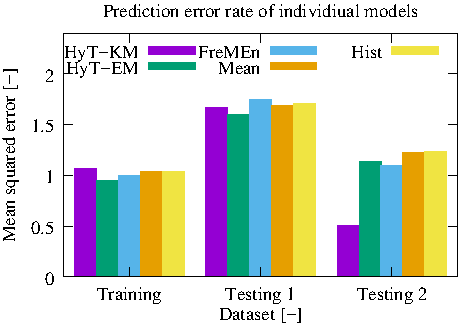
\includegraphics[width=0.24\columnwidth]{fig/nav_graph}
%      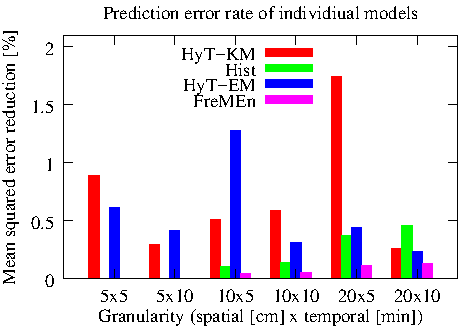
\includegraphics[width=0.24\columnwidth]{fig/ped_graph}
%      \caption{Predicted people occurrence over a T-shaped corridor during different parts of the day. Screen grab from the video available at~\url{https://youtu.be/4SW4j7DDxYE}.\label{fig:video}}
%      \caption{Predicted people occurrence over a T-shaped corridor, see video at \url{https://youtu.be/4SW4j7DDxYE}.\label{fig:video}}
%   \end{center}
%\end{figure}

\begin{figure}[!b]
   \begin{center}
      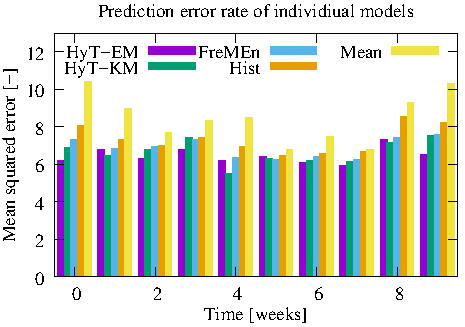
\includegraphics[width=0.45\columnwidth]{fig/door_graph}
    \hfill
      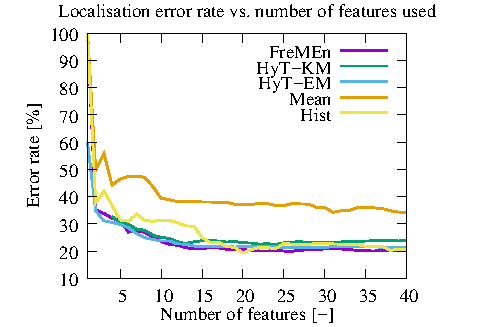
\includegraphics[width=0.45\columnwidth]{fig/localisation_graph}\\\vspace{5mm}
      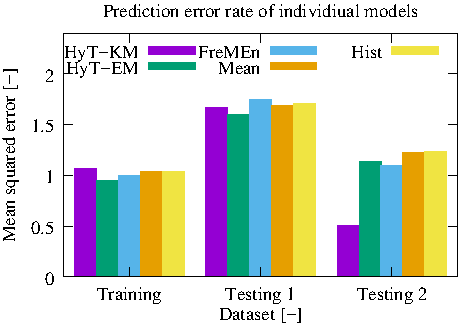
\includegraphics[width=0.45\columnwidth]{fig/nav_graph}
    \hfill
      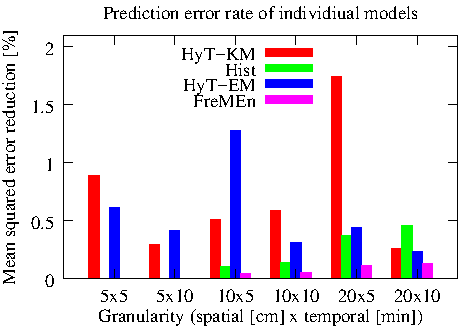
\includegraphics[width=0.45\columnwidth]{fig/ped_graph}
    \caption{Four different scenarios for autonomous robot decision-making. We tested five methods: \textit{Mean}, which predicts the average value of measurements over the whole time line in every spatial cell, \textit{Hist}, which predicts average of every hour of the day in every spatial cell, \textit{FreMEn}, which creates temporal model for every spatial cell, \textit{HyT-EM} which creates spatio-temporal model using EM GMM for clustering and brute force to find proper parameters of the model (number of clusters and the dimensionality of the warped hypertime), \textit{HyT-KM} which creates spatio-temporal model using our specialized clustering method and tries to estimate proper parameters of the model (for more details, please see \cite{krajnik2018warped}).\\
\textbf{Top left:} the prediction of the door state during different weeks,\\
\textbf{top right:} the prediction of the most probably visible points of interest in the specific times,\\
\textbf{bottom left:} the prediction of the time to travers the path in the specific times,\\
\textbf{bottom right:} the prediction of the frequency of people on the T-shaped junction using different resolution - prediction power of \textit{Hist}, \textit{FreMEn}, \textit{HyT-EM} and \textit{HyT-KM} are compared to the prediction power of \textit{Mean} to better visualize the impact of using different methods.
\label{fig:complexControl}}
   \end{center}
\end{figure}

Based on the experiments described in the \cite{krajnik2018warped}, see Figure \ref{fig:complexControl}, we can say that the methods using warped hypertime on the one-dimensional time series are not performing better than FreMEn.
However, it seems that in the more complex scenarios, like the human presence experiment, the predictive power of the warped hypertime based methods start to excel.
It should be noted, that even prediction of anomalous behaviour [mesas] using one-dimensional binary variable was
enough complex scenario to prove better prediction power of the \makebox{WHyTe-powered} methods.

To verify the hypothesis that warped hypertime space methods will predict better than discrete ones, we need to create more scenarios using more complex variables.
In these days we are working on the new, better-controlled dataset of human presence in cooperation with Environment Perception and Autonomous Navigation research group at the Universite de Technologie de Belfort-Montbeliard.
Moreover, we are preparing new scenarios from other sources.



